\newcommand{\CC}{\cellcolor{Gray}}
\definecolor{Gray}{gray}{0.9}

\subsection{Experimental Evaluation of Conservative Data Sharing}
\label{sec:exp}

We conduct experiments to answer six main questions: \textbf{(1)} can \cdsmethodname\ prevent performance degradation when sharing data as observed in Section~\ref{sec:analysis}?, \textbf{(2)} how does \cdsmethodname\ compare to vanilla multi-task offline RL methods and prior data sharing methods?
\textbf{(3)} can \cdsmethodname\ handle sparse reward settings, where data sharing is particularly important due to scarce supervision signal? \textbf{(4)} can \cdsmethodname\ handle goal-conditioned offline RL settings where the offline dataset is undirected and highly suboptimal? \textbf{(5)} Can \cdsmethodname\ scale to complex visual observations? \arxiv{\textbf{(6)} Can \cdsmethodname\ be combined with any offline RL algorithms? Besides these questions, we visualize CDS weights for better interpretation of the data sharing scheme learned by CDS in Figure~\ref{fig:antmaze_vis} in Appendix~\ref{app:cds_vis}}.

\begin{wrapfigure}{r}{0.45\textwidth}
    \vspace{-0.65cm}
    \centering
    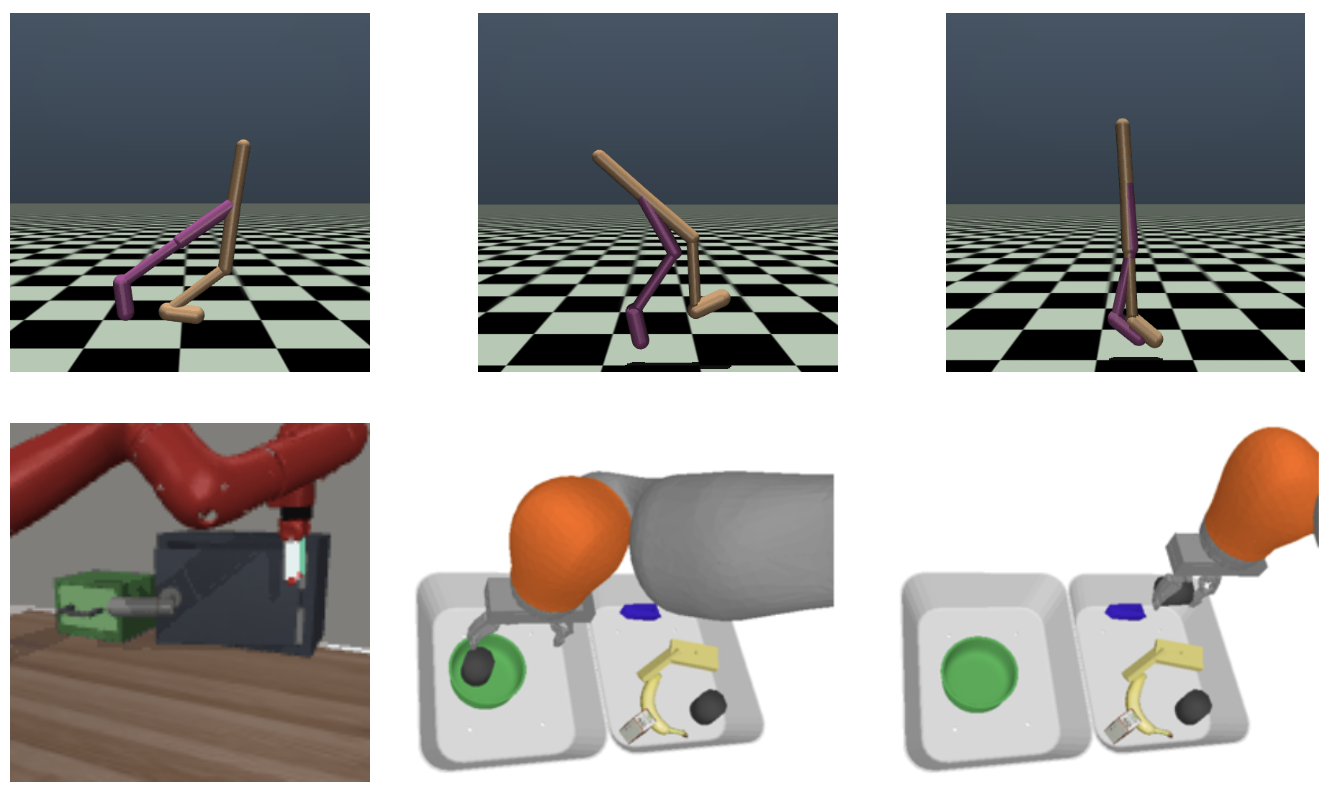
\includegraphics[width=0.95\linewidth]{chapters/cds/env.png}
    \vspace{-0.32cm}
    \caption{\footnotesize  Environments (from left to right): walker2d {run forward}, walker2d {run backward}, walker2d {jump},  Meta-World {door open/close} and {drawer open/close} and vision-based pick-place tasks in \citep{kalashnikov2021mt}.}
    \label{fig:env}
    \vspace{-0.4cm}
\end{wrapfigure}
\textbf{Comparisons.} To answer these questions, we consider the following prior methods. On tasks with low dimensional state spaces, we compare with the online multi-task relabeling approach \textbf{HIPI}~\citep{eysenbach2020rewriting}, which uses inverse RL to infer for which tasks the datapoints are optimal and in practice routes a transition to task with the highest Q-value. We adapt HIPI to the offline setting by applying its data routing strategy to a conservative offline RL algorithm.
We also compare to na\"ively sharing data across all tasks (denoted as \textbf{Sharing All}) and vanilla multi-task offline RL method without any data sharing (denoted as \textbf{No Sharing}). On image-based domains, we compare \cdsmethodname\ to the data sharing strategy based on human-defined skills~\citep{kalashnikov2021mt} (denoted as \textbf{Skill}), which manually groups tasks into different skills (e.g. skill ``pick'' and skill ``place'') and only routes an episode to target tasks that belongs to the same skill.
In these domains, we also compare to \textbf{HIPI}, \textbf{Sharing All} and \textbf{No Sharing}. \arxiv{Beyond these multi-task RL approaches with data sharing, to assess the importance of data sharing in offline RL, we perform an additional comparison to other alternatives to data sharing in multi-task offline RL settings. One traditionally considered approach is to use data from other tasks for some form of ``pre-training'' before learning to solve the actual task. We instantiate this idea by considering a method from \citet{yang2021representation} that conducts contrastive representation learning on the multi-task datasets to extract shared representation between tasks and then runs multi-task RL on the learned representations. We discuss this comparison in detail in Table~\ref{tbl:pretrain_comparison} in Appendix~\ref{app:pretrain_comparison}.} 
To answer question (6), we use CQL~\citep{kumar2020conservative} (a Q-function regularization method) and BRAC~\citep{wu2019behavior} (a policy-constraint method) as the base offline RL algorithms for all methods. \arxiv{We discuss evaluations of CDS with CQL in the main text and include the results of CDS with BRAC in Table~\ref{tbl:brac_comparison} in Appendix~\ref{app:brac_results}.} For more details on setup and hyperparameters, see Appendix~\ref{app:details}.


\textbf{Multi-task environments.} We consider a number of multi-task reinforcement learning problems on environments visualized in Figure~\ref{fig:env}. 
% To answer questions (1) and (2), we consider three locomotion environments from OpenAI Gym~\citep{brockman2016openai} with dense rewards: halfcheetah, walker2d, and ant. Each environment has three tasks, \texttt{run forward}, \texttt{run backward} and \texttt{jump}, as used in prior offline RL work~\citep{yu2020mopo}.
{To answer questions (1) and (2), we consider the walker2d locomotion environment from OpenAI Gym~\citep{brockman2016openai} with dense rewards. We use three tasks, \texttt{run forward}, \texttt{run backward} and \texttt{jump}, as proposed in prior offline RL work~\citep{yu2020mopo}.}
To answer question (3), we also evaluate on robotic manipulation domains using environments from the Meta-World benchmark~\citep{yu2020metaworld}. We consider four tasks: \texttt{door open}, \texttt{door close}, \texttt{drawer open} and \texttt{drawer close}. Meaningful data sharing requires a consistent state representation across tasks, so we put both the door and the drawer on the same table, as shown in Figure~\ref{fig:env}. Each task has a sparse reward of 1 when the success condition is met and 0 otherwise. To answer question (4), we consider maze navigation tasks where the temporal ``stitching'' ability of an offline RL algorithm is crucial to obtain good performance. We create goal reaching tasks using the ant robot in the medium and hard mazes from D4RL~\citep{fu2020d4rl}. The set of goals is a fixed discrete set of size 7 and 3 for large and medium mazes, respectively. Following \citet{fu2020d4rl}, a reward of +1 is given and the episode terminates if the state is within a threshold radius of the goal. Finally, to explore how \cdsmethodname\ scales to image-based manipulation tasks (question (5)), we utilize a simulation environment similar to the real-world setup presented in~\citep{kalashnikov2021mt}. This environment, which was utilized by \citet{kalashnikov2021mt} as a representative and realistic simulation of a real-world robotic manipulation problem, consists of 10 image-based manipulation tasks that involve different combinations of picking specific objects (banana, bottle, sausage, milk box, food box, can and carrot) and placing them in one of the three fixtures (bowl, plate and divider plate) (see example task images in Fig.~\ref{fig:env}).
More environment details are in the appendix. We report the average return for locomotion tasks and success rate for AntMaze and both manipluation environments, averaged over 6 and 3 random seeds for environments with low-dimensional inputs and image inputs respectively.

\begin{table}[h]
\vspace{0.1cm}
  \centering
  \scriptsize
  \def\arraystretch{0.9}
  \setlength{\tabcolsep}{0.42em}
  \vspace{-0.4cm}
\resizebox{0.95\linewidth}{!}{\begin{tabular}{cc|cccc}
  \toprule
 \multicolumn{1}{c}{\multirow{1.5}[2]{*}{Environment}} & \multicolumn{1}{c}{\multirow{1.5}[2]{*}{Dataset types / Tasks}}\vline &
 \multicolumn{3}{c}{$D_\text{KL}(\pi, \pi_\beta)$}\\
& \multicolumn{1}{c}{} \vline& \multicolumn{1}{c}{\textbf{No Sharing}}  & \multicolumn{1}{c}{\textbf{Sharing All}} & \multicolumn{1}{c}{\textbf{CDS (basic) (ours)}}  & \multicolumn{1}{c}{\textbf{CDS (ours)}}\\
\midrule
  &medium-replay / run forward & \textbf{1.49} & 7.76 & 14.31 & \textbf{1.49}\\
  walker2d& medium / run backward &  \textbf{1.91} & 12.2 & 8.26 & 6.09\\
  %\rowcolor{Gray}
  & \cellcolor{yellow} expert / jump & \cellcolor{yellow} 3.12 & \cellcolor{yellow} 27.5 & \cellcolor{yellow} 13.25  & \cellcolor{yellow} \textbf{2.91}\\
    \bottomrule
    \end{tabular}}
    \vspace{0.1cm}
         \caption{\footnotesize Measuring $D_\text{KL}(\pi, \pi_\beta)$ on the walker2d environment.  \textbf{Sharing All} degrades the performance on task \text{jump} with limited expert data as discussed in Table~\ref{tab:analysis}. \cdsmethodname\ manages to obtain a $\behavior$ after data sharing that is closer to the single-task optimal policy in terms of the KL divergence compared to \textbf{No Sharing} and \textbf{Sharing All} on task \texttt{jump} (highlighted in yellow). Since \cdsmethodname\ also achieves better performance, this analysis suggests that reducing distribution shift is important for effective offline data sharing.
     \label{tab:analysis_cds}
     \vspace{-0.3cm}
     }
\end{table}

\textbf{Multi-task datasets.}  Following the analysis in Section~\ref{sec:analysis}, we intentionally construct datasets with a variety of heterogeneous behavior policies to test if \cdsmethodname\ can provide effective data sharing to improve performance while avoiding harmful data sharing that exacerbates distributional shift. For the locomotion domain, we use a large, diverse dataset (medium-replay) for \texttt{run forward}, a medium-sized dataset for \texttt{run backward}, and an expert dataset with limited data for \texttt{run jump}. For Meta-World, we consider medium-replay datasets with 152K transitions for task \texttt{door close} and \texttt{drawer open} and expert datasets with only 2K transitions for task \texttt{door open} and \texttt{drawer close}. For AntMaze, we modify the D4RL datasets for antmaze-*-play environments to construct two kinds of multi-task datasets: an ``undirected'' dataset, where data is equally divided between different tasks and the rewards are correspondingly relabeled, and a ``directed'' dataset, where a trajectory is associated with the goal closest to the final state of the trajectory. This means that the per-task data in the undirected setting may not be relevant to reaching the goal of interest. Thus, data-sharing is crucial for good performance: methods that do not effectively perform data sharing and train on largely task-irrelevant data are expected to perform worse. Finally, for image-based manipulation tasks, we collect datasets for all the tasks individually by running online RL~\cite{kalashnikov2018scalable} until the task reaches medium-level performance (40\% for picking tasks and 80\% placing tasks). At that point, we merge the entire replay buffers from different tasks creating a final dataset of 100K RL episodes with 25 transitions for each episode.

\begin{table*}[t!]
\centering
\vspace*{0.1cm}
\scriptsize
\resizebox{\textwidth}{!}{\begin{tabular}{l|l|r|r|r|r|r}
\toprule
\textbf{Environment} & \textbf{Tasks / Dataset type} & \textbf{\cdsmethodname\ (ours)} & \textbf{\cdsmethodname\ (basic)} & \textbf{HIPI}~\cite{eysenbach2020rewriting}& \textbf{Sharing All} & \textbf{No Sharing}\\ \midrule
% & run forward / medium-replay & 2587.7  & \textbf{2626.1} & 2605.0 & \textbf{2632.5}\\
% halfcheetah & run backward / medium & 2519.5  & \textbf{2634.4} & \textbf{2636.7} & \textbf{2630.7}\\
% & jump / expert & \textbf{4298.2} & 4113.4 & 712.3 & -1978.3\\
% & \CC \textbf{average} & \CC \textbf{3135.1} & \CC \textbf{3124.7} & \CC 1984.7 & \CC 1095.0\\
% \midrule
& run forward / medium-replay & \textbf{1057.9}$\pm$121.6 & 968.6$\pm$188.6 & 695.5$\pm$61.9 & 701.4$\pm$47.0 & 590.1$\pm$48.6\\
walker2d & run backward / medium & 564.8$\pm$47.7 & 594.5$\pm$22.7 & 626.0$\pm$48.0& \textbf{756.7}$\pm$76.7& 614.7$\pm$87.3\\
& jump / expert & 1418.2$\pm$138.4 & 1501.8$\pm$115.1  & \textbf{1603.7}$\pm$146.8 & 885.1$\pm$152.9 & 1575.2$\pm$70.9\\
& \CC \textbf{average} & \CC 1013.6$\pm$71.5 &\CC \textbf{1021.6}$\pm$76.9 & \CC 975.1$\pm$45.1 & \CC 781.0$\pm$100.8 & \CC 926.6$\pm$37.7\\\midrule
% & run forward / medium-replay & 2350.1 & \textbf{2658.9} & 1175.0 & 2126.7\\
% ant & run backward / medium & 1435.7 & 1208.2 & 1488.7 & \textbf{2021.7}\\
% & jump / expert & \textbf{2781.3} & 2670.4 & 133.8 & 495.8\\
% & \CC \textbf{average} & \CC \textbf{2189.0} & \CC \textbf{2179.2} & \CC 932.5 & \CC 1548.1\\
% \midrule
& door open / expert & \textbf{58.4\%}$\pm$9.3\% & 30.1\%$\pm$16.6\% & 26.5\%$\pm$20.5\% & 34.3\%$\pm$17.9\% & 14.5\%$\pm$12.7\\
& door close / medium-replay & \textbf{65.3\%}$\pm$27.7\% & 41.5\%$\pm$28.2\% & 1.3\%$\pm$5.3\% & 48.3\%$\pm$27.3\% & 4.0\%$\pm$6.1\% \\
Meta-World~\citep{yu2020metaworld}& drawer open / medium-replay & \textbf{57.9\%}$\pm$16.2\% & 39.4\%$\pm$16.9\% & 41.2\%$\pm$24.9\% & 55.1\%$\pm$9.4\% & 16.0\%$\pm$17.5\%\\
& drawer close / expert & 98.8\%$\pm$0.7\% & 86.3\%$\pm$0.9\% & 62.2\%$\pm$33.4\% & \textbf{100.0\%}$\pm$0\% & 99.0\%$\pm$0.7\%\\
& \CC \textbf{average} & \CC \textbf{70.1\%}$\pm$8.1\% & \CC 49.3\%$\pm$16.0\% & \CC 32.8\%$\pm$18.7\% & \CC 59.4\%$\pm$5.7\% & \CC 33.4\%$\pm$8.3\%\\
\midrule
& large maze (7 tasks) / undirected & \textbf{22.8}\% $\pm$ 4.5\% & 10.0\% $\pm$ 5.9\% & 1.3\% $\pm$ 2.3\%  & 16.7\% $\pm$ 7.0\% & 13.3\% $\pm$ 8.6\% \\
AntMaze~\citep{fu2020d4rl}  & large maze (7 tasks) / directed &  \textbf{24.6\%} $\pm$ 4.7\% & 0.0\% $\pm$ 0.0\% & 11.8\% $\pm$ 5.4\% & 20.6\% $\pm$ 4.4\% & 19.2\% $\pm$ 8.0\% \\
& medium maze (3 tasks) / undirected &  \textbf{36.7\%} $\pm$ 6.2\% & 0.0\% $\pm$ 0.0\% & 8.6\% $\pm$ 3.2\% & 22.9\% $\pm$ 3.6\% & 21.6\% $\pm$ 7.1\% \\
& medium maze (3 tasks) / directed &  \textbf{18.5}\% $\pm$ 6.0\% & 0.0\% $\pm$ 0.0\% & 8.3\% $\pm$ 9.1\% & 12.4\% $\pm$ 5.4\% & \textbf{17.0\%} $\pm$ 3.2\% \\
\bottomrule
\end{tabular}}
\vspace{-0.2cm}
\caption{\footnotesize Results for multi-task locomotion (walker2d), robotic manipulation (Meta-World) and navigation environments (AntMaze) with low-dimensional state inputs.
% On the locomotion environment walker2d, we include three tasks with different styles of datasets, \texttt{run forward} + a medium replay dataset, \texttt{run backward} + a medium dataset and \texttt{jump} + an expert dataset with limited data. On the multi-task robotic manipulation domain, we consider four tasks from Meta-World~\citep{yu2020metaworld}, door open, door close, drawer open and drawer close with medium-replay, expert, medium-replay and expert datasets respectively.
% % Similar to locomotion tasks, we also used limited amount of expert trajectories for the expert dataset.
% On the antmaze navigation task, we consider two maze layouts (medium/large) from D4RL~\citep{fu2020d4rl} with the directed and undirected datasets.
 \arxiv{Numbers are averaged across 6 seeds, $\pm$ the 95$\%$-confidence interval.} We include per-task performance for walker2d and Meta-World domains and the overall performance averaged across tasks (highlighted in gray) for all three domains. We bold the highest score across all methods. \cdsmethodname\ achieves the best or comparable performance on all of these environments.
}
\label{tbl:gym}
\normalsize
\vspace{-0.3cm}
\end{table*}
%%AK: things seemed a bit diverging with CDS (basic) on antmaze, I guess it is fine for now since it is not the main method, but we could revisit back later during camera-ready.

\begin{table*}[t!]
\small{
\centering
\vspace*{0.1cm}
\resizebox{\textwidth}{!}{\begin{tabular}{l|r|r|r|r|r}
\toprule
\textbf{Task Name} & \textbf{\cdsmethodname\ (ours)}& \textbf{HIPI}~\cite{eysenbach2020rewriting} & \textbf{Skill~\cite{kalashnikov2021mt}} & \textbf{Sharing All} & \textbf{No Sharing}\\ \midrule
\texttt{lift-banana} & \textbf{53.1\%}$\pm$3.2\% & 48.3\%$\pm$6.0\%  & 32.1\%$\pm$9.5\% & 41.8\%$\pm$4.2\% & 20.0\%$\pm$6.0\%\\
\texttt{lift-bottle} & \textbf{74.0\%}$\pm$6.3\% & 64.4\%$\pm$7.7\%  & 55.9\%$\pm$9.6\% & 60.1\%$\pm$10.2\% & 49.7\%$\pm$8.7\%\\
\texttt{lift-sausage} & \textbf{71.8\%}$\pm$3.9\%  & 71.0\%$\pm$7.7\%  & 68.8\%$\pm$9.3\% & 70.0\%$\pm$7.0\% & 60.9\%$\pm$6.6\%\\
\texttt{lift-milk}& \textbf{83.4\%}$\pm$5.2\% & 79.0\%$\pm$3.9\% & 68.2\%$\pm$3.5\% & 72.5\%$\pm$5.3\% & 68.4\%$\pm$6.1\%\\

\texttt{lift-food} & 61.4\%$\pm$9.5\% & \textbf{62.6\%}$\pm$6.3\% & 41.5\%$\pm$12.1\% & 58.5\%$\pm$7.0\% & 39.1\%$\pm$7.0\%\\
\texttt{lift-can} & 65.5\%$\pm$6.9\% & \textbf{67.8\%}$\pm$6.8\%  & 50.8\%$\pm$12.5\% & 57.7\%$\pm$7.2\% & 49.1\%$\pm$9.8\%\\
\texttt{lift-carrot} & \textbf{83.8\%}$\pm$3.5\% & 78.8\%$\pm$6.9\% & 66.0\%$\pm$7.0\%& 75.2\%$\pm$7.6\%& 69.4\%$\pm$7.6\%\\
\texttt{place-bowl} & \textbf{81.0\%}$\pm$8.1\%  & 77.2\%$\pm$8.9\% & 80.8\%$\pm$6.9\% & 70.8\%$\pm$7.8\% & 80.3\%$\pm$8.6\%\\
\texttt{place-plate} & 85.8\%$\pm$6.6\%  & 83.6\%$\pm$7.9\% & 78.4\%$\pm$9.6\% & 78.7\%$\pm$7.6\% & \textbf{86.1}\%$\pm$7.7\%\\
\texttt{place-divider-plate} & \textbf{87.8\%}$\pm$7.6\%  & 78.0\%$\pm$10.5\% & 80.8\%$\pm$5.3\% & 79.2\%$\pm$6.3\% & 85.0\%$\pm$5.9\%\\
%\midrule
\CC \textbf{average} & \CC \textbf{74.8\%}$\pm$6.4\%  & \CC 71.1\%$\pm$7.5\% & \CC 62.3\%$\pm$8.9\% & \CC 66.4\%$\pm$7.2\% & \CC 60.8\%$\pm$7.5\%\\
\bottomrule
\end{tabular}}
\vspace{-0.1cm}
\caption{\footnotesize Results for multi-task vision-based robotic manipulation from \citep{kalashnikov2021mt}. \arxiv{Numbers are averaged across 3 seeds, $\pm$ the 95$\%$ confidence interval.} We consider 7 tasks denoted as \texttt{lift-object} where the goal of each task is to lift a different object and 3 tasks denoted as \texttt{place-fixture} that aim to place a lifted object onto different fixtures. \cdsmethodname\ outperforms both a skill-based data sharing strategy~\citep{kalashnikov2021mt} (\textbf{Skill}) and other data sharing methods on the average success rate (highlighted in gray) and 7 out of 10 per-task success rates.
}
\label{tbl:mtopt}
}
\vspace{-0.6cm}
\end{table*}


% \subsection{Evaluating CDS on Multi-Task Offline RL}
\textbf{Results on domains with low-dimensional states.} We present the results on all non-vision environments in Table~\ref{tbl:gym}.
% , but leave the results of halfcheetah and ant to Appendix~\ref{app:additional_exp}. 
\cdsmethodname\ achieves the 
best average performance across all environments except that on walker2d, it achieves the second best performance, obtaining slightly worse the other variant \cdsmethodname\ (basic). On the locomotion domain, we observe the most 
significant improvement on task \texttt{jump} on all three environments. We interpret this as strength of conservative data sharing, which mitigates the distribution shift that can be introduced by routing large amount of other task data to the task with limited data and narrow distribution. We also validate this by measuring the $D_\text{KL}(\pi, \pi_\beta)$ in Table~\ref{tab:analysis_cds} where $\pi_\beta$ is the behavior policy after we perform \cdsmethodname\
to share data. As shown in Table~\ref{tab:analysis_cds}, \cdsmethodname\ achieves lower KL divergence
 between the single-task optimal policy and the behavior policy after data sharing on task \texttt{jump} with limited expert data, whereas \textbf{Sharing All} results in much higher KL divergence compared to \textbf{No Sharing} as discussed in Section~\ref{sec:analysis} and Table~\ref{tab:analysis}. Hence, \cdsmethodname\ is able to mitigate distribution shift when sharing data and result in performance boost.


On the Meta-World tasks, we find that the agent without data sharing completely fails to solve most of the tasks due to the low quality of the medium replay datasets and the insufficient data for the expert datasets. \textbf{Sharing All} improves performance since in the sparse reward settings, data sharing can introduce more supervision signal and help training. \cdsmethodname\ further improves over \textbf{Sharing All}, suggesting that \cdsmethodname\ can not only prevent harmful data sharing, but also lead to more effective multi-task learning compared to \textbf{Sharing All} in scenarios where data sharing is imperative. It's worth noting that \cdsmethodname\ (basic) performs worse than \cdsmethodname\ and \textbf{Sharing All}, indicating that relabeling data that only mitigates distributional shift is too pessimistic and might not be sufficient to discover the shared structure across tasks.

%\textbf{Goal-conditioned AntMazes~\citep{fu2020d4rl}.} 

On AntMaze, we observe that \cdsmethodname\ performs better than \textbf{Sharing All} and significantly outperforms HIPI in all four settings. Perhaps surprisingly, \textbf{No Sharing} is a strong baseline, however, is outperformed by \cdsmethodname\ with the harder undirected data. Moreover, \cdsmethodname\ performs on-par or better in the undirected setting compared to the directed setting, indicating the effectiveness of \cdsmethodname\ in routing data in challenging settings. 




% Concretely, we consider three different styles of datasets in gym domains: medium-replay for \texttt{run forward}, medium for \texttt{run backward}, and expert for \texttt{run jump}, following the convention proposed in \citep{fu2020d4rl}.

% Since it is common to generate a large number of data from multiple policies with different levels of performance, we use 120K, 120K and 250K datapoints 
% %%CF.5.22: are you referring to different checkpoints or different #s of datapoints?
% %%TY.5.26: I mean different number of datapoints.
% medium-replay datasets in halfcheetah, walker2d and ant respectively. Meanwhile, it is usually time-consuming to collect medium or high quality data in the real world and thus we provide 25K, 25K and 50K datapoints for medium datasets and 5K, 5K and 20K datapoints for expert datasets for the aforementioned three environments respectively.
% As analyzed in Section~\ref{sec:analysis} and Table~\ref{tab:analysis}, na\"ively sharing data across all tasks would hurt multi-task performance when behavior policies differ in each task. To test if \cdsmethodname\ can mitigate this issue, we adopt medium-replay datasets for task \texttt{run forward}, medium datasets for task \texttt{run backward} and expert datasets for task \texttt{jump}.










% \subsection{Results on image-based robotic manipulation tasks}
% \label{sec:mtopt_results}

\textbf{Results on image-based robotic manipulation domains.}  %\textbf{Skill} manually defines two oracle skills ``picking'' and ``placing'' and shares all picking tasks share data with each other but does not share data with any of the placing tasks and vice-versa. 
Here, we compare \cdsmethodname\ to the hand-designed \textbf{Skill} sharing strategy, in addition to the other methods. \arxiv{Given that \cdsmethodname\ achieves significantly better performance than \cdsmethodname\ (basic) on low-dimensional robotic manipulation tasks in Meta-World, we only evaluate \cdsmethodname\ in the vision-based robotic manipulation domains.}  Since \cdsmethodname\ is applicable to any offline multi-task RL algorithm, we employ it as a separate data-sharing strategy in \citep{kalashnikov2021mt} while keeping the model architecture and all the other hyperparameters constant, which allows us to carefully evaluate the influence of data sharing in isolation. The results are reported in Table~\ref{tbl:mtopt}. \cdsmethodname\ outperforms both \textbf{Skill} and other approaches, indicating that \cdsmethodname\ is able to scale to high-dimensional observation inputs and can effectively remove the need for manual curation of data sharing strategies.

